\chapter{Galoistheorie}


Im Folgenden sei $K$ ein Körper, $\_K$ ein fest gewählter algebraischer Abschluss von $K$ und alle algebraischen Erweiterungskörper $E$ von $K$ seien als Unterkörper von $\_K$ gewählt, d.h. $K \subset E \subset \_K$, also $\_E = \_K$.


\section{Separabilität}


\begin{df} \label{19.1-1}
	Ein Polynom $f \in K[x]$ vom Grad größer gleich 1 heißt \emphdef[separabel]{separabel über $K$}, falls $f$ keine mehrfachen Nullstellen in $\_K$ besitzt, d.h. $f = \lambda (x - \alpha_1) \dotsc (x - \alpha_n) \in \_K[x]$ mit $\alpha_1, \dotsc, \alpha_n \in \_K$ paarweise verschieden, $\lambda \in \_K$, $n = \deg f$.
	\begin{note}
		Für $K \subset E \subset \_K$ und $f \in K[x]$ separabel über $K$, ist auch $f$ separabel über $E$.
	\end{note}
\end{df}

\begin{df} \label{19.1-2}
	Sei $f = \lambda_0 + \lambda_1 x + \lambda_2 x^2 + \dotsc + \lambda_n x^n \in K[x]$, $\lambda_n \neq 0$.
	Dann heißt das Polynom
	\[
		\ddx f = f' = \lambda_1 + 2 \lambda_2 + \dotsb + i \lambda_i x^{i-1} + \dotsb + n \lambda_n x^{n-1}
		\in K[x]
	\]
	\emphdef{formale Ableitung} von $f$.
\end{df}

\begin{lem}[Produktregel] \label{19.1-3}
	Die Abbildung $\ddx: K[x] \to K[x] : f \mapsto \ddx f$ ist $K$-linear und es gilt
	\[
		\ddx (fg) = (\ddx f) g + f (\ddx g)
	\]
	für alle $f, g \in K[x]$.
	Abbildungen von $K$-Algebren, die $K$-linear sind und die obige Produktregel erfüllen, heißen \emphdef{Derivationen}.
\end{lem}

\begin{lem} \label{19.1-4}
	Sei $f \in K[x], \deg f \ge 1$ und sei $\alpha \in \_K$ eine Nullstelle von $f$.
	Dann ist $\alpha$ mehrfache Nullstelle von $f$ (in $\_K$, $f \in K[x] \subset \_K[x]$) genau dann, wenn $\alpha$ auch Nullstelle (in $\_K$) von $f' = \ddx f$ ist, d.h. wenn $f'(\alpha) = 0$.
\end{lem}

\begin{kor} \label{19.1-5}
	$\alpha \in \_K$ ist genau dann mehrfache Nullstelle von $f \in K[x] \subset \_K[x]$, $\deg f \ge 1$, wenn $\alpha$ Nullstelle von $\ggT(f, f') \in K[x]$ ist.
\end{kor}

\begin{kor} \label{19.1-6}
	Sei $f \in K[x], \deg f \ge 1$.
	Dann ist $f$ separabel genau dann, wenn $\ggT(f, f') = 1$ ist.
\end{kor}

\begin{kor} \label{19.1-7}
	Sei $f \in K[x]$ irreduzibel.
	Dann ist $f$ separabel genau dann, wenn $\ddx f = f' \neq 0$ ist.
\end{kor}

Wann kann es passieren, dass $\ddx f$ das Nullpolynom ist?

Sei $f = \sum_{i=0}^n \lambda_i x^i, \lambda_n \neq 0, n \ge 1$.
Dann ist $f' = \ddx f = \sum_{i=0}^n i \lambda_i x^{i-1} = 0 \in K[x]$ genau dann, wenn $i \lambda_i = 0$ ist für alle $i \in \{1, \dotsc, n\}$.
\begin{seg}{1. Fall: $\Char K = 0$}
	In dem Fall ist $\lambda_i = 0$ für alle $i \in \{1, \dotsc, n\}$, d.h. $f$ ist ein konstantes Polynom.
\end{seg}
\begin{seg}{2. Fall: $\Char K = p > 0$}
	Dann ist $\lambda_i = 0$ für alle $1 \le i \le n$, die nicht von $p$ geteilt werden.
	Teilt $p$ den Index $i$, so ist für beliebige $\lambda_i$ stets $i \lambda_i = 0$, da $i \equiv 0 \bmod p$ ist.
	Also ist $f$ von der Form
	\[
		f = \lambda_0 + \lambda_p x^p + \lambda_{2p} x^{2p} + \dotsb + \lambda_{kp} x^{kp} \in K[x],
	\]
	d.h. $f(x) = g(x^p)$ mit $g(x) = \lambda_0 + \mu_1 x + \dotsb + \mu_k x^k$ mit $\mu_i = \lambda_{ip}$, $i \in \{1, \dotsc, k\}$.
	Insbesondere ist dann $n = \deg f = kp = p \deg g$.
\end{seg}

Im Lichte von \ref{19.1-7} haben wir gezeigt:

\begin{st} \label{19.1-8}
	Sei $f \in K[x]$ irreduzibel, also insbesondere $\deg f \ge 1$.
	Dann gilt
	\begin{enumerate}[i)]
		\item
			Ist $\Char K = 0$, dann ist $f$ separabel.
		\item
			Ist $\Char K = p > 0$, dann ist $f$ inseparabel genau dann, falls es ein Polynom $g \in K[x]$ gibt mit $f(x) = g(x^p)$.
			Insbesondere ist dann $\deg f = p \deg g$.
	\end{enumerate}
	Ist $f(x) = g(x^p)$ in ii) irreduzibel, $f(x) = g(x^p)$, so ist $g \in K[x]$ ebenfalls irreduzibel.
\end{st}

\begin{df} \label{19.1-9}
	Sei $\alpha \in \_K$.
	Dann heißt $\alpha$ \emphdef[separabel!Element]{separabel über $K$}, falls das Minimalpolynom $\mu_{\alpha, K} \in K[x]$ separabel ist.
	Ein algebraischer Erweiterungskörper $E$ von $K$, (d.h. $K \subset E \subset \_K$) heißt \emphdef{separabel über $K$}, falls $\alpha$ separabel für $K$ ist für alle $\alpha \in E$.
	Ein Körper $K$ heißt \emphdef{vollkommen} (engl. “perfect”), falls jede algebraische Erweiterung von $K$ separabel über $K$ ist
\end{df}

\setcounter{thm}{5}
\begin{kor} \label{19.1-6}
	\begin{enumerate}[i)]
		\item
			Körper der Charakteristik $0$ sind vollkommen.
		\item
			Algebraische Erweiterungen vollkommener Körper sind vollkommen.
		\item
			Endliche Körper sind vollkommen.
	\end{enumerate}
\end{kor}

\begin{ex} \label{19.1-7}
	Konstruiere eine einfache nicht separable Körpererweiterung (\ref{19.1-6} wird vorausgesetzt): $K \subset K(\alpha) \subset \_K$.
\end{ex}

\begin{lem} \label{19.1-8}
	Seien $K \subset E \subset L \subset \_K$ Körper und sei $L$ separabel über K.
	Dann ist $L$ auch separabel über $E$.
\end{lem}

\begin{nt} \label{19.1-9}
	$\alpha \in \_K$ ist separabel genau dann, wenn $\alpha \in \_K$ Nullstelle eines separablen Polynoms $f \in K[x]$ ist, denn dann teilt $\mu_{\alpha, K}$ das Polynom $f$ und ist daher separabel.
\end{nt}

\begin{df} \label{19.1-10}
	Seien $K \subset E, L \subset \_K$ Körper.
	Die Menge der $K$-Homomorphismen von $E$ nach $L$ wird mit $\Hom_{K-\text{Alg}}(E, L)$ bezeichnet.
	Der \emphdef[Separabilitätsgrad]{Separabilitätsgrad $[E : K]_S$ von $E$ über $K$} ist definiert als $|\Hom_{K-\text{Alg}}(E, \_K)|$, ist also die Anzahl der verschiedenen $K$-linearen Körperhomomorphismen von $E$ nach $\_K$.
\end{df}

\begin{lem} \label{19.1-11}
	Sei $E = K(\alpha), \alpha \in \_K$.
	Dann ist $[E : K]_S$ die Anzahl der verschiedenen Nullstellen von $\mu_{\alpha, K} \in K[x]$ in $\_K$.
\end{lem}

\begin{kor} \label{19.1-12}
	Sei $\alpha \in \_K$.
	Dann ist $\alpha$ separabel über $K$ genau dann, wenn $[K(\alpha) : K]_S = [K(\alpha) : K]$ ist.
\end{kor}

\begin{st} \label{19.1-13}
	Seien $K \subset E \subset L \subset \_K$ Körper.
	Dann ist $[L : K]_S = [L : E]_S [E : K]_S$.
\end{st}

\begin{lem} \label{19.1-14}
	Sei $K \subset E \subset \_K, [E : K] < \infty$.
	ist $E$ separabel über $K$, so ist $[E : K]_S = [E : K]$.
\end{lem}

Um die Umkehrung von \ref{19.1-14} zu beweisen, brauchen wir noch mehr Informationen über inseparabel Körpererweiterungen.

Die folgende Definition ist grundlegend für Körper der Charakteristik $p > 0$.

\begin{df} \label{19.1-15}
	Sei $\Char K = p > 0$.
	Die Abbildung $\scr F = \scr F_p: K \to K: \alpha \mapsto \alpha^p$ heißt \emphdef{Frobeniushomomorphismus} von $K$.
	Ist $k \in \N, q = p^k$, so wird die $k$-fache Iteration $\scr F_p \circ \scr F_p \circ \dotsb \circ \scr F_p = (\scr F_p)^k$ mit $\scr F_q$ bezeichnet.
\end{df}

\begin{st}[Freshman's Dream] \label{19.1-16}
	Sei $\Char K = p > 0$.
	Dann ist $\scr F_p: K \to K$ ein Körperhomomorphismus und $\scr F_p\big|_{\GF(p)} = \id_{\GF(p)}$, wobei $\GF(p)$ der Primkörper von $K$ ist.
\end{st}

\begin{kor} \label{19.1-17}
	Sei $K$ endlicher Körper mit Primkörper $\GF(p) = \F_p$.
	Dann ist $\scr F: K \to K: \alpha \mapsto \alpha^p$ ein $\F_p$-Automorphismus von $K$.
\end{kor}

\begin{lem} \label{19.1-18}
	Sei $\Char K = p > 0$ und sei $f \in K[x]$ irreduzibel.
	Sei $r \in \N_0$ maximal, sodass es ein $g \in K[x]$ mit $f(x) = g(x^{p^r})$ gibt.
	Dann hat jede Nullstelle von $f$ in $\_K$ Vielfachheit $p^r$ und $g \in K[x]$ ist irreduzibel und separabel.
	Die Nullstellen von $f$ sind genau die $p^r$-ten Wurzeln der Nullstellen von $g$, und diese Wurzeln sind eindeutig in $\_K$.
\end{lem}

\begin{st} \label{19.1-19}
	Sei $E$ eine endliche Körpererweiterung von $K$, d.h. $[E : K] < \infty$.
	Dann ist $E \subset \_K$ und es gilt:
	$E$ ist separabel über $K$ genau dann, wenn $[E : K]_S = [E : K]$ ist.
\end{st}

\begin{st} \label{19.1-20}
	Seien $K \subset E \subset L$ Körper.
	Dann ist $L$ genau dann separabel über $K$, wenn $L$ über $E$ und $E$ über $K$ separabel sind.
\end{st}


\section{\texorpdfstring{$K^*$}{K*}, endliche Körper, Satz von primitiven Element}

$K^* = K \setminus \{0\}$ bildet bezüglich der Multiplikation eine abelsche Gruppe.
Es gilt:

\begin{st} \label{19.2-1}
	Sei $G$ eine endliche Untergruppe von $K^*$.
	Dann ist $G$ zyklisch.
\end{st}

\begin{st} \label{19.2-2}
	Sei $|K| < \infty$.
	Dann ist $\Char K = p > 0$ für eine Primzahl $p$, $|K| = q = p^k$ für ein $k \in \N$ und $K^*$ zyklisch von der Ordnung $q - 1$.
\end{st}

Jetzt können wir eine vollständige Klassifizierung aller endlichen Körper liefern.

\begin{st} \label{19.2-3}
	Sei $p \in \N$ Primzahl, $q = p^n$ ($n \in \N$) eine Potenz von $p$.
	Sei $\Z / p\Z = \GF(p) = \F_p$ der (eindeutig bestimmte) Körper mit $p$ vielen Elementen.
	Dann gibt es einen bis auf $\F_p$-Isomorphismen eindeutigen Erweiterungskörper $\F_q$ von $\F_p$ mit $q$ vielen Elementen und es existiert ein $\zeta \in \F_q$ so, dass $\F_q = \F_p(\zeta)$ gilt (d.h. $\F_q$ ist einfache, wegen $[\F_q : \F_p] = n$ algebraische Erweiterung mit primitiven Element $\zeta \in \F_q$).
\end{st}

\begin{kor} \label{19.2-4}
	Seien $K$ und $E$ endlicher Körper.
	Dann ist $K$ isomorph zu einem Unterkörper von $E$ genau dann, wenn $\Char K = \Char E = p > 0$ ist und $|K| = p^k, |E| = p^n$ mit $k, n \in \N, k \divs n$ gilt.
\end{kor}

\begin{kor} \label{19.2-5}
	Endliche Körper sind perfekt.
\end{kor}

\begin{st}[Satz vom primitiven Element]
	Sei $K \subset E$ endliche, separable Körpererweiterung.
	Dann existiert ein primitives Element $\alpha \in E$ mit $E = K(\alpha)$.
	$E$ ist also einfache Körpererweiterung von $K$.
\end{st}


\section{Zerfällungskörper}


\begin{df} \label{19.3-1}
	Sei $\scr F = \{ f_i : i \in I \} \subset K[x]$ eine Menge von nicht konstanten Polynomen in $K[x]$ für eine Indexmenge $I$.
	Ein Erweiterungkörper $E$ von $K$ heißt \emphdef[Zerfällungskörper]{Zerfällungskörper von $\scr F$ über $K$}, wenn gilt
	\begin{enumerate}[i)]
		\item
			Jedes $f_i, i \in I$ zerfällt in $E[x]$ vollständig in Linearfaktoren.
		\item
			Die Erweiterung $K \subset E$ wird von den Nullstellen der $f_i, i \in I$ erzeugt.
	\end{enumerate}
\end{df}

Ein Zerfällungskörper $E$ von $\scr F$ ist also algebraisch über $K$ nach \ref{18.3-8}.
Ist $\scr F = \{f\}$, $f \in K[x], \deg f \ge 1$, so ist der Zerfällungskörper von $\scr F$ über $K$ die Körpererweiterung $E = K(\alpha_1, \dotsc, \alpha_n)$, wobei $\alpha_1, \dotsc, \alpha_n$ die Nullstellen von $f$ in $\_K$ seien.
Wir sagen: „$E$ ist der Zerfällungskörper von $f$“.
Allgemein mit $\scr F = \{ f_i : i \in I\}$ ist der Zerfällungskörper von $\scr F$ über $K$ offensichtlich $E = K(\alpha_j : j \in J)$, wobei $\alpha_j \in \_K$ alle Nullstellen der Polynome $f_i, i \in I$ durchläuft.
Ist $\scr F = \{ f_1, f_2, \dotsc, f_n \}$, so ist der Zerfällungskörper $E$ von $\scr F$ über $K$ gerade der Zerfällungskörper des Polynoms $g = f_1 f_2 \dotsb f_n \in K[x]$ über $K$.

\begin{st} \label{19.3-2}
	Sei $E$ algebraische Körpererweiterung von $K$.
	Dann sind die folgenden Aussagen äquivalent:
	\begin{enumerate}[i)]
		\item
			Ist $\tau: E \to \_E = \_K$ ein $K$-Homomorphismus, so ist $\im \tau = E$ (hier ist tatsächlich Gleichheit gemeint, $\im \tau \isomorphic E$ gilt immer).
		\item
			Jedes irreduzible Polynom aus $K[x]$, das in $E$ eine Nullstelle besitzt, zerfällt in $E[x]$ in Linearfaktoren.
		\item
			$E$ ist Zerfällungskörper einer Menge nicht konstanter Polynome in $K[x]$.
	\end{enumerate}
\end{st}

\begin{df} \label{19.3-3}
	Eine algebraische Körpererweiterung $E$ von $K$ heißt \emphdef[normal]{normal über $K$}, falls $E$ die äquivalenten Bedingungen von \ref{19.3-2} erfüllt.
\end{df}

\begin{note}
	Ist $[E : K] = 2$, so ist $E$ stets normal über $K$.
\end{note}

\begin{kor} \label{19.3-4}
	Seien $K \subset E \subset L \subset \_K$ Körper und sei $L$ normal über $K$.
	Dann ist $L$ normal über $E$.
	\begin{proof}
		nach \ref{19.3-2} iii).
	\end{proof}
\end{kor}

\begin{note}
	$K \subset E \subset L$ mit $L$ normal über $E$ und $E$ normal über $K$ impliziert nicht, dass $L$ normal über $K$ ist.
	Mit anderen Worten: „normal über“ ist nicht transitiv.
\end{note}

\begin{df} \label{19.3-5}
	Seien $K \subset E \subset \_K$ Körper.
	Eine \emphdef{normale Hülle} $L$ von $E$ über $K$ ist eine algebraische, normale Erweiterung von $K$, die $E$ enthält und so, dass kein Zwischenkörper $E \subset L \subsetneq L$ normal über $K$.
\end{df}

\begin{note}
	Ist $E$ normal über $K$, so ist $E$ normale Hülle von $E$ über $K$.
\end{note}

\begin{st} \label{19.3-6}
	Sei $K \subset E \subset \_K$.
	Dann existiert eine normale Hülle $L$ von $E$ (in $\_K$) und diese ist eindeutig bestimmt.
	Ist $[E : K]$ endlich, so auch $[L : K]$.
\end{st}

\begin{ex} \label{19.3-7}
	Sei $K = \Q$.
	$f(x) = x^3 - 2 \in \Q[x]$ ist irreduzibel (Eisenstein mit $p = 2$).
	Dann sind $\alpha := \sqrt[3]{2}, \beta := \sqrt[3]{2} e^{i\f{2\pi}3}$ und $\gamma := \sqrt[3]{2} e^{i\f{4\pi}3}$ die drei Nullstellen von $f$ in $\_{\Q}[x]$ und
	\[
		\Q[x] / (x^3-2)\Q[x] \isomorphic \Q(\sqrt[3]{2}) = E \subset \R.
	\]
	Insbesondere ist $E$ nicht normal über $\Q$, da $\sqrt[3]{2} e^{i\f{2\pi}3} \not\in \R$ ist.
	Nach \ref{18.4-4} sind die Körper $\Q(\alpha), \Q(\beta), \Q(\gamma)$ $K$-isomorph (in $\_\Q$ enthalten), aber nicht gleich in $\_{\Q}$.
	Der Zerfällungskörper von $f$ über $\Q$ ist 6-dimensional.
\end{ex}


\section{Der Hauptsatz der Galoistheorie}


Unser Ziel ist jetzt, einen Zusammenhang zwischen Körpererweiterungen $K \subset E$ und den „Symmmetriegruppen“ $\Aut_K(E)$ (Menge aller $K$-Automorphismen auf $E$) herzustellen.

\begin{df} \label{19.4-1}
	Sei $K \subset E$ Körpererweiterung.
	Die Menge der $K$-Automorphismen von $E$ bildet bezüglich der Komposition von Abbildungen eine Gruppe, die \emphdef{Galoisgruppe} $G(E/K)$ von $E$ über $K$.
\end{df}

Das Beispiel \ref{19.3-7} zeigt, dass es durcheaus passieren kann, dass $G(E/K) = \{ \id_E \}$ ist, auch wenn $E$ eine echte Körpererweiterung von $K$ ist:
Für $E = \Q(\sqrt[3]{2}) \subset \R$ muss jeder $\Q$-Automorphismus von $E$ die relle Wurzel $\sqrt[3]{2}$ in sich abbilden und ist daher die Identität von $E$ (mit \ref{18.4-4}).
In diesem Fall enthält $G(\Q(\sqrt[3]{2}/\Q)$ keine Information über die Körpererweiterung!
Um solche Fälle zu vermeiden, werden wir fordern, dass die Körpererweiterung $K \subset E$ über $K$ normal ist (wir beschränken uns auf algebraische Erweiterungen).

\begin{df} \label{19.4-2}
	Eine algebarische, separable und normale Körpererweiterung $E$ von $K$ heißt \emphdef[Galoiserweiterung]{Galoiserweiterung von $K$} oder \emphdef[galoissch]{galoissch über $K$}.
\end{df}

\begin{nt} \label{19.4-3}
	Sei $\sigma$ ein Körperautomorphismus von $K$.
	Wegen $\sigma(1_K) = 1_K$ und $\sigma(z 1_K) = z \sigma(1_K) = z 1_K$ für alle $z \in \Z$ ist $\sigma|_\Pi = \id_\pi$, wobei $\Pi$ der Primkörper von $K$ ist.
	So ist immer $G(K / \Pi) = \Aut(K)$.
\end{nt}

\begin{st} \label{19.4-4}
	Sei $E$ endliche, normale Erweiterung von $K$.
	Dann ist $|G(E/K)| = [E:K]_S \le [E:K]$.
\coursetimestamp{30}{05}{2014}
	\begin{proof}
		Sei $K \subset E \subset \_K = \_E$.
		Sei $\sigma: E \to \_K$ $K$-Homomorphismus, dann ist $\im \sigma = E$ nach \ref{19.3-2} i) da $E$ normal über $K$ ist.
		So erhalten wir durch Einschränkeen des Bildbereichs eine Bijektion von $\Hom_K(E, \_K)$ auf $\Aut_K(K) = G(E/K)$.
		Daher ist
		\[
			|G(E / K)| = | \Hom_K(E, \_K)| = [E : K]_S
		\]
		nach \ref{19.1-10}.
		Da $[E : K] < \infty$ ist, finden wir $\alpha_1, \dotsc, \alpha_n \in E$ so, dass $E = K(\alpha_1, \dotsc, \alpha_n)$ ist.
		Sei $L_i = K(\alpha_1, \dotsc, \alpha_i)$, $i \in \{1, \dotsc, n\}$, so ist $L_i = L_{i-1}(\alpha_i)$ und daher $[L_i : L_{i-1}]_S \le [L_i : L_{i-1}]$ mit \ref{19.1-11}.
		Mit \ref{19.1-13} und \ref{18.1-2} folgt
		\[
			[E:K]_S = [E : L_{n-1}]_S \dotsb [L_1 : K]_S
			\le [E : L_{n-1}] \dotsb [L_1 : K]
			= [E : K].
		\]
	\end{proof}
\end{st}

Direkt aus \ref{19.1-14} und \ref{19.4-4} folgt nun

\begin{kor} \label{19.4-5}
	Sei $E$ endlich und galoissch über $K$.
	Dann ist $|G(E/K)| = [E:K]$.
\end{kor}

\begin{ex} \label{19.4-6}
	Sei $p$ eine Primzahl, $n = md \in \N$ und $q_1 = p^m, q_2 = p^n$, sowie $\F_1 = \F_{q_1}, \F_2 = \F_{q_2}$.
	Dann ist $\F_p \subset \F_p \subset \F_2 \subset \_{\F_p}$.
	Da endliche Körper perfekt sind (nach \ref{19.2-5}) ist $\F_2$ separabel über $\F_1$.
	Weiter besteht $\F_2$ aus den Nullstellen von $x^{q_2} - x \in \F_p[x] \subset \F_1[x]$ und ist daher Zerfällungskörper von $x^{q_1} - x$ über $\F_1$, also normal über $\F_1$ (\ref{19.2-3} und \ref{19.3-2}).

	Also ist $\F_2$ galoisch über $\F_1$ und daher gilt mit \ref{19.4-5} $|G(\F_2 / \F_1)| = [\F_2 : \F_1] = d$ (wegen $|\F_1|^d = q_1^d = (p^m)^d = p^n = q_2 = |\F_2|$).

	Erinnerung:
	Der Frobeniushomomorphismus $\scr F: \_{\F_p} \to \_{\F_p}: \alpha \to \alpha^P$ induziert durch Einschränken $\F_p$-Automorphismen von $\F_1$ und $\F_2$ nach \ref{19.1-17}.

	Setze $\scr F_{q_1} = (\scr F)^m: \F_2 \to \F_2: \alpha \mapsto \alpha^{q_1}$.
	Wegen $\alpha^{q_1} = \alpha$ für alle $\alpha \in \F_1$ (da $\alpha \in \F_1$ Nullstelle von $x^{q_1} - x \/n \F_p[x]$ ist, siehe Beweis von \ref{19.2-3}) ist $\scr F_{q_1}$ ein $\F_1$ Automorphismus von $\scr F_2$, d.h. $\scr F_{q_1}\big|_{\F} = \id_{\F_1}$.

	Sei $\zeta \in \F_2$ Erzeuger von $\F_2^*$, so ist $|\zeta| = q_2 - 1$.
	Insbesondere ist $\scr F_{q_1}(\zeta) = \zeta^{q_1} \neq \zeta$ und $\scr F_{q_1}^d(\zeta) = \zeta^{q_1^{d}} = \zeta^{q_2} = \zeta$ und daher ist $(\scr F_{q_1})^d = \id_{\F_2}$, d.h. $\scr F_{q_1}$ ist ein nicht triviales Element in $G(\F_2 / \F_1)$ der Ordnung $d$, da $d$ minimal mit $\zeta^{q_1^{d}} = \zeta$ ist.
	Wir haben gezeigt: $G(\F_2 / \F_1) = \< \scr F_{q_1} \>$ ist zyklisch der Ordnung $d$.
\end{ex}

\begin{conv} \label{19.4-7}
	Sei $E$ endliche, galoische Erweiterung von $K$.
	Dann ist $G(E / K)$ endlich der Ordnung $[E: K]$.
	$E$ heißt abelsche, zyklische, auflösbare, \dots, Erweiterung, falls $G(E / K)$ abelsch, bzw. zyklisch, bzw. auflösbar, \dots ist.
\end{conv}

\begin{df} \label{19.4-8}
	Sei $E$ ein Körper und $G$ eine Gruppe von Körperautomorphismen von $E$, d.h. $G \le \Aut(E) = \Aut_{\Pi(E)}(E) = G(E / \Pi(E))$.
	Dann ist
	\[
		E^G := \{\alpha \in E \;|\; \forall \sigma \in G : \sigma(\alpha) = \alpha\}
	\]
	die Menge der Fixpunkte von $E$ unter $G$.
	Ist $K \subset E$ und $G \le G(E / K)$, so ist offensichtlich $K \subset E^G$.
\end{df}

\begin{lem} \label{19.4-9}
	Sei $E$ ein Körper und $G \le \Aut(E)$.
	Dann ist $E^G$ ein Unterkörper von $E$, der \emphdef[Fixkörper]{Fixkörper von $E$ unter $G$}.
	\begin{note}
		Ist $K \subset E$, $G \le G(E / K)$, so gilt $K \subset E^G \subset E$.
	\end{note}
	\begin{proof}
		Wegen $0, 1_E \in E^G$ ist $E^G \neq (0)$.
		Seien $\alpha, \beta \in E^G$, so ist $\sigma(\alpha \pmd \beta) = \sigma(\alpha) \pmd \sigma(\beta) = \alpha \pmd \beta$ für alle $\sigma \in G$.
		Für $\alpha \neq 0$ ist dann $(\sigma(\alpha))^{-1} = \sigma(\alpha^{-1})$.
		Also sind $\alpha \pmd \beta, \alpha^{-1} \in E^G$, d.h. $E^G$ ist ein Körper $\subset E$.
	\end{proof}
\end{lem}

\begin{lem} \label{19.4-10}
	Seien $K \subset E$ Körper, $H \le G \le G(E / K)$.
	Dann ist $E^G \subset E^H$.
	So ist $G \mapsto E^G$ eine inklusionsumkehrende Abbildung von der Menge der Untergruppen $G$ von $G(E / K)$ in die Menge der Zwischenkörper $K \subset L \subset E$.
	\begin{proof}
		Sei $\alpha \in E^G$, so ist $\sigma(\alpha) = \alpha$ für alle $\sigma \in G$ und daher ist erst recht $\sigma(\alpha) = \alpha$ für alle $\sigma \in H \subset G$.
		Also ist $\alpha \in E^H$ und daher ist $E^G \subset E^H$.
		Klar ist auch $K \subset E^G \subset E^H \subset E$.
	\end{proof}
\end{lem}

\begin{lem} \label{19.4-11}
	Sei $E$ galoissch über $K$ und sei $L$ mit $K \subset L \subset E$ ein Zwischenkörper.
	Dann ist $E$ galoissch über $L$ und $G(E / L) \le G(E / K)$.

	Sind $K \subset L_1 \subset L_2 \subset E$ Zwischenkörper, so ist $G(E / L_2) \le G(E / L_1) \le G(E / K)$.
	Insbesondere ist $G(E / ?): L \mapsto G(E / L)$ eine inklusionsumkehrende Abbildung von der Menge der Zwischenkörper $L$, $K \subset L \subset E$ in die Menge der Untergruppen von $G(E / K)$.
	\begin{proof}
		Wegen \ref{19.1-8} ist $E$ separabel über $L$ und wegen \ref{19.3-4} ist $E$ normal über $L$.
		Also ist $E$ galoissch über $L$.
		Jeder $L$-Automorphismus von $E$ ist natürlich auch $K$-Automorphismus und daher in $G(E / K)$ enthalten.
		Also ist $G(E / L) \le G(E / K)$.

		Jeder $L_2$-Automorphismus von $E$ ist erst recht $L_1$-Automorphismus und daher $G(E / L_2) \subset G(E / L_1)$.
	\end{proof}
\end{lem}

\begin{conv} \label{19.4-12}
	Seien $K \subset E \subset \_K = \_E$ Körpererweiterungen, $G = G(E / K) = \Aut_K(E)$.
	Wir setzen $\scr U := \{ H \le G \}, \scr Z = \{ L : K \subset L \subset E, L\text{ Körper } \}$.
	Dann sind $\scr U$ und $\scr Z$ durch Inklusion teilweise geordnete Mengen.
	Wir haben Abbildungen
	\begin{enumerate}[i)]
		\item
			$E^? : \scr U \to \scr Z : H \mapsto E^H \subset E$,
		\item
			$G(E / \argdot): \scr Z \to \scr U : L \mapsto G(E / L) \le G$.
	\end{enumerate}
	Beide Abbildungen sind inklusionsumkehrend (und funktionieren auch ohne die Voraussetzung, dass $E$ galoissch über $K$ ist).
\end{conv}

Unser Ziel ist die Aussage:
Ist $E$ galoissch und endlich über $K$, so sind $E^?$ und $G(E / \argdot)$ invers zueinander und daher injektiv.

\begin{st} \label{19.4-13}
	Sei $E$ galoissch über $K$, $K \subset E \subset \_K = \_E$.
	Dann ist $E^? \circ G(E / \argdot) : \scr Z \to \scr Z : L \mapsto E^{G(E / L)}$ die Identität auf $\scr Z$, d.h. es gilt für alle Zwischenkörper $L$ mit $K \subset L \subset E$ die Aussage
	\[
		E^{G(E / L)} = L.
	\]
	Insbesondere ist $E^{G(E/K)} = K$.
	Mit anderen Worten: „Der Fixkörper unter der Galoisgruppe $G(E / L)$ von $E$ ist $L$.“
	\begin{proof}
		Sei $L \in \scr Z$, so ist $K \subset L \subset E \subset \_K = \_E = \_L$.
		Da $E$ galoissch über $K$ ist, ist es auch galoissch über $L$ nach \ref{19.1-20}.
		Sei $H := G(E / L) \le G(E / K)$.
		Zu zeigen ist $E^H = L$.
		Sei $\tau \in H, \alpha \in L$, dann ist wegen $\tau|_L = \id|_L$ gerade $\tau(\alpha) = \alpha$, d.h. $L \subset L^H$.
		Sei $\alpha \in E^H$, dann ist also $K \subset L \subset L(\alpha) \subset E^H \subset E \subset \_K$.
		Sei $\tau$ irgendeine $L$-Einbettung von $L$ in $\_K = \_L$.
		Nach dem Fortsetzungssatz \ref{18.4-7} existiert $\hat \tau: E \to \_K$ mit $\hat \tau|_{L(\alpha)} = \tau$.
		Da $E$ normal über $K$ ist und $\Hom_L(E, \_K) \subset \Hom_K (E, \_K)$ ist $\im \hat \tau = E$.
		Also ist $\hat \tau \in \Aut_L(E) = G(E / L) = H$.
		Aber $\tau(\alpha) = \alpha$ und wir haben gezeigt, dass es nur eine $L$-Einbettung von $L(\alpha)$ in $\_K = \_L$ gibt.
		Also ist $[L(\alpha) : L]_S = 1$.
		Wegen $L(\alpha) \subset E$ ist $\alpha$ separabel über $L$ und daher ist $[L(\alpha) : L] = [L(\alpha) : L]_S = 1$ nach \ref{19.1-12}.
		Also ist $\alpha \in L$ und daher ist $E^H = L$.
	\end{proof}
\end{st}

\begin{kor} \label{19.4-14}
	Sei $E$ galoissch über $K$, $K \subset E \subset \_K$.
	Dann ist die Abbildung $G(E / \argdot): \scr Z \to U : L \mapsto G(E / L) \le G(E / K)$ injektiv und $E^? : \scr U \to \scr : H \mapsto E^H$ für $H \le G(E / K)$ ist surjektiv.
	\begin{proof}
		Sind allgemein $\psi \circ \phi = \id$ Abbildungen, dann ist $\psi$ surjektiv und $\phi$ injektiv.
	\end{proof}
\end{kor}

Wir untersuchen jetzt, wann ein Zwischenkörper $L \in \scr Z$ mit $K \subset L \subset E$ selbst galoisch über $K$ ist unter der Generalvoraussetzung, dass $E$ galoissch über $K$ ist.

Sei also $L \in \scr Z$ und $K \subset E \subset \_K = \_E$ galoissche Erweiterung.
Sei $\sigma \in G(E / K)$.
Ist $K \subset L \subset E$ ein Zwischenkörper, so ist $\sigma(L)$ ebenfalls ein solcher, wegen $K = \sigma(K) \subset \sigma(L) \subset \sigma(E) = E$.
Dann gilt

\begin{st} \label{19.4-15}
	Sei $L \in \scr Z$, $\sigma \in G(E / K)$, $H = G(E / L)$.
	Dann ist $G(E / \sigma(L)) = \sigma H \sigma^{-1}$, die zu $H$ (mit $\sigma$) \emphdef{konjugierte Untergruppe} von $G(E / K)$.
	\begin{proof}
		$\sigma H = \sigma H \sigma^{-1} = \{ \sigma \tau \sigma^{-1} : \tau \in H \} \le G$.
		Ist $\tau \in G(E / K)$, so ist $\tau \in G(E / L) \iff \tau(\alpha) = \alpha$ für alle $\alpha \in L$ und $\rho \in G(E / \sigma(L)) \iff \rho(\sigma(\alpha)) = \sigma(\alpha) \iff \sigma^{-1}\rho\sigma(\alpha) = \alpha \iff \sigma^{-1}\rho\sigma \in H \iff \rho \in \sigma H \sigma^{-1}$ für alle $\alpha \in L$.
	\end{proof}
\end{st}

\begin{nt} \label{19.4-16}
	Sind $K \subset E \subset \_K = \_E$ Körper und ist $E$ normal über $K$ und $\iota: E \to \_K$ die natürliche Einbettung, so definiert $\tau \to \iota \circ \tau : E \to \_K$ eine Bijektion zwischen $\Aut_K(E) = G(E / K)$ und $\Hom_K(E, \_K)$.
	Dies ist so, weil nach \ref{19.3-2} i) das Bild $\im \rho = E \subset \_K$ ist für alle $\rho \in \Hom_K (E, \_K)$ und daher die Abbildung $\tau \mapsto \iota \circ \tau$ surjektiv ist.
	Wir können also $\tau \in G(E / K)$ mit $\iota \circ \tau$ identifizieren, d.h. $\tau \in G(E / K)$ als $K$-Homomorphismus von $E$ in $\_K = \_E$ betrachten.

	Die Umkehrabbildung um aus einem $\rho \in \Hom_K(E, \_K)$ ein $\rho \in G(E / K)$ zu machen fuktioniert durch Beschränken des Bildbereichs.
\end{nt}

\begin{st} \label{19.4-17}
	Sei $E$ galoissche Körpererweiterung von $K$ und $L \in \scr Z$.
	So ist $K \subset L \subset E \subset \_K = \_E = \_L$.
	Seien $G = G(E / K)$ und $H = G(E / L) \le G$.
	Dann ist $L$ galoissch über $K$ genau dann, wenn $H$ normale Untergruppe von $G$ ist.
	In diesem Fall ist $\sigma(L) = L$ für alle $\sigma \in G$ und die Abbildung $\tau \mapsto \tau|_L$ ($\tau \in G$) ist ein Gruppenepimorphismus von $G$ auf $G(L / K)$ mit Kern $H$.
	So ist
	\[
		G(L / K) \isomorphic G(E / K) / G(E / L) = G / H.
	\]
	\begin{proof}
		\begin{segnb}[$\implies$]
			Sei $L$ galoissch über $K$.
			Dann ist für $\tau \in \Hom_K(E, \_K) = G$, $\tau|_L \in \Hom_K(L, \_K)$ und daher ist $\im \tau|_L = L$ nach \ref{19.3-2} i), da nach Voraussetzung $L$ normal über $K$ ist.
			Also ist $\tau|_L \in G(L / K) = \Hom_K(L, \_K)$.
			Klar ist für $\tau, \sigma \in G$ ist $\tau|_L \circ \sigma|_L = (\tau \circ \sigma)|_L$.
			Also ist $\tau \mapsto \tau|_L$ ein Gruppenhomomorphismus von $G$ in $G(L / K)$.
			Darüber hinaus ist $\tau|_L = \id|_L$ genau dann, wenn $\tau \in G(E / L)$.
			Also ist $G(E / L) = \ker(\tau \mapsto \tau|_L)$.
			Also ist $H = G(E / L) \Idealof G = G(E / K)$.
			(Alternativ gilt nach \ref{19.4-15}: $H = G(E / L) = G(E / \tau(L)) = \tau H = \tau H \tau^{-1}$ für alle $\tau \in G$).

			Sei $\sigma \in G(L / K) = \Hom_K(L, \_K)$.
			Nach \ref{18.4-7} ergibt sich
			\[
				\begin{tikzcd}
					E \arrow{rrd}{\exists \hat \sigma} \\
					L \arrow[inj]{u} \arrow{r}{\sigma} & L \arrow[inj]{r} & \_K
				\end{tikzcd},
			\]
			es existiert also $\hat \sigma$ mit $\hat \sigma|_L = \sigma$.
			Es ist $\sigma(E) = E$, da $E$ normal über $K$ ist.
			Also ist $\hat \sigma \in G$ und $\hat \sigma|_L = \sigma = G(L / K)$.
			Also ist $\tau \mapsto \tau|_L$ ein Gruppenepimorphismus von $G(E / K)$ auf $G(L / K)$ mit $\ker H = G(E / L)$.
			Also ist $G(L / K) \isomorphic G / H$ nach dem ersten Isomorphiesatz.
		\end{segnb}
		\begin{segnb}{$\impliedby$}
			Sei $G(E / L) = H \Idealof G = G(E / K)$.
			$L$ ist separabel über $K$ nach \ref{19.1-20}.
			Es bleibt zu zeigen, dass $L$ normal über $K$ ist.
			Nach \ref{19.3-2} genügt es zu zeigen, dass $\im \sigma = L$ für alle $\sigma \in \Hom_K(L, \_K)$.
			Sei $\sigma \in \Hom_K(L, \_K)$.
			Mit \ref{18.4-7},
			\[
				\begin{tikzcd}
					E \arrow{rd}{\exists \hat \sigma} \\
					L \arrow[inj]{u}{\iota} \arrow{r}{\sigma} & K
				\end{tikzcd}
			\]
			existiert $\hat\sigma \in \Hom_K(E, \_K)$ mit $\hat \sigma|_L = \sigma$.
			Also ist $\hat\sigma(E) = E$ ($E$ galoissch über $K$), d.h. $\hat \sigma \in G = G(E / K)$.
			Nun ist $\sigma H \sigma^{-1} = H$, da $H \Idealof G$ ist.
			Mit \ref{19.4-13} und \ref{19.3-15} haben wir
			\[
				L
				\stack{\ref{19.4-13}}= E^{G(E / L)}
				= E^H
				= E^{\sigma H}
				\stack{\ref{19.4-15}}= E^{G(E / \sigma(L))}
				= \sigma(L).
			\]
			Also ist für alle $\sigma \in G$ gerade $\sigma(L) = L$, d.h. $L$ ist galoissch über $K$.
		\end{segnb}
	\end{proof}
\end{st}

\coursetimestamp{02}{06}{2014}

\begin{st}[Artin] \label{19.4-18}
	Sei $E$ algebraische Erweiterung von $K$ und sei $H \le \Aut_K(E) = G(E / K)$.
	Sei $L = E^H$ der Fixkörper unter $H$.
	Dann ist $E$ galoissch über $L$ und $H \le G(E / L)$.
	Ist darüber hinaus $H$ eine endliche Gruppe, so ist $H = G(E / L)$ und $[E : L] = |H| < \infty$.
	\begin{proof}
		$E$ ist algebraisch über $K$, also auch algebraisch über $L$.
		Wir müssen zeigen: $E$ ist separabel und normal über $K$.

		Sei $\alpha \in E$, $p = \mu_{\alpha, L} \in L[x]$.
		Für alle $\sigma \in H$ haben wir dann: $\sigma(p) = p$, da die Koeffizienten von $p$ Elemente des Fixkörpers $L = E^H$ sind, siehe \ref{18.4-3}.
		Seien $\sigma_1, \dotsc, \sigma_r \in H$ so gewählt, dass die $\sigma_i(\alpha)$ für $i \in \{1, \dotsc, r\}$ paarweise verschieden sind und für jedes $\tau \in H$ ein $i \in \{1, \dotsc, r\}$ existiert mit $\tau(\alpha) = \sigma_i(\alpha)$.
		Da $1_H(\alpha) = \alpha$ ist $\alpha \in \{\sigma_1(\alpha), \dotsc, \sigma_r(\alpha)\}$.
		Sei $\tau \in H$, dann ist $\{\tau\sigma_1(\alpha), \dotsc, \tau\sigma_r(\alpha)\} = \{ \sigma_1(\alpha), \dotsc, \sigma_r(\alpha) \}$, d.h. $\tau$ permutiert die Menge $\{\sigma_1(\alpha), \dotsc, \sigma_r(\alpha) \}$.
		Beachte: $\sigma_i(\alpha) \in E$ für $i \in \{1, \dotsc, r\}$, da $\sigma_i \in H \le G(E / K)$.
		Sei
		\[
			h := \prod_{i=1}^r (x - \underbrace{\sigma_i(\alpha)}_{\in E}) \in E[x].
		\]
		Dann ist für $\tau \in H$: $\tau(h) = \prod_{i=1}^r (x - \tau \sigma_i(\alpha))	= \prod_{i=1}^r (x - \sigma_i(\alpha)) = h$.
		Also ist $h \in L[x]$ und damit ist $p$ Teiler von $h$, da $h(\alpha) = 0$ ist ($\exists i: \alpha = \sigma_i(\alpha))$.
		Andererseits ist nach Konstruktion $h$ ein Teiler von $p$.
		Also ist $h = p = \mu_{\alpha, L}$, d.h. $\alpha$ ist separabel über $L$, da $h$ nur Nullstellen mit Vielfachheit $1$ besitzt.
		Also ist $E$ separabel über $L$.

		Darüber hinaus zerfällt $h = \mu_{\alpha, L} \in L[x]$ in $E$ in Linearfaktoren und daher ist $E$ der Zerfällungskörper aller Polynome $\mu_{\alpha, L} \in L[x]$ über $L$ und daher normal über $L$.

		Also ist $E$ galoissch über $L$.
		Per definitionem $L = E^H$ gilt $H \le G(E / L)$.

		Sei nun $|H| = n < \infty$ und $\alpha \in E$.
		Dann hat $H\alpha = \{ \tau(\alpha) : \tau \in H \}$ höchstens $n$ viele Elemente.
		Daher ist $\deg \mu_{\alpha, L} = r = \deg h \le n$ nach dem oben Gezeigten. 
		Also ist $[L(\alpha) : L] = \deg \mu_{\alpha, K} \le n$ für alle $\alpha \in E$.
		Sei $L \subset M \subset E$ ein beliebiger Zwischenkörper mit $[M: L] < \infty$.
		Da $E$ separabel über $L$ ist, ist $M$ separabel über $K$ nach \ref{19.1-20} und daher existiert nach \ref{19.2-6} ein primitives Element für $M$, d.h. $M = L(\alpha)$ für ein $\alpha \in M$.
		Also ist $[M : L] \le n$.
		Sei $M = L(\alpha)$ ein über $L$ endlich-dimensionaler Zwischenkörper ($L \subset M \subset E$) maximaler Dimension.
		Dann gilt also für alle $\beta \in E$: $[M(\beta) : L] \le [M : L]$ und daher ist $M(\beta) \subset M$, d.h. $\beta \in M$.
		Also ist $E = M = L(\alpha)$ und $[L(\alpha) : L] \le n$.
		Mit \ref{19.4-4} ist aber $n = |H| = \le |G(E/L)| = [E:L]_S = [E : L]$ und daher ist $[E : L] = n$ und $G(E / L) = H$.
	\end{proof}
\end{st}

\begin{kor} \label{19.4-19}
	Sei $E$ algebraisch über $K$.
	Dann ist $E$ galoissch über $K$ genau dann, wenn $E^{G(E / K)} = K$ ist.
	\begin{proof}
		\begin{segnb}{$\implies$}
			Sei $E$ galoissch über $K$, so ist $E^{G(E/K)} = K$ nach \ref{19.4-13}.
		\end{segnb}
		\begin{segnb}{$\impliedby$}
			Nach \ref{19.4-18}.
		\end{segnb}
	\end{proof}
\end{kor}

\begin{kor} \label{19.4-20}
	Sei $K \subset E \subset \_K$ mit $E$ galoissch und endlich über $K$.
	Dann ist $G(E / \argdot) \circ E^? = \id_{\scr U}$, wobei $\scr U = \{ H \le G(E / K) \}$ definiert war.
	\begin{proof}
		Zu zeigen: ist $H \le G = G(E / K)$, so ist $G(E / \argdot) \circ E^? (H) = G(E / \argdot) (E^H)0= G(E / E^H) = H$.
		Nach \ref{19.4-5} ist $G(E / K) = [E : K] < \infty$.
		Also ist $|H| < \infty$ und $E$ ist galoissch über $E$ mit Galoisgruppe $H$ nach \ref{19.4-18}.
	\end{proof}
\end{kor}

\begin{kor}[Hauptsatz der Galoistheorie für endliche Körpererweiterungen] \label{19.4-21}
	Sei $K \subset E \subset \_K$ galoissch und sei $[E : K] < \infty$.
	Sei $G = G(E / K), \scr U = \{H \le G\}, \scr Z = \{ K \subset L \subset E \}$.
	Dann ist $[E : K] = |G|$ und die Abbildungen
	\begin{align*}
		E^?: \scr U &\to \scr Z: H \mapsto E^H, \\
		G(E / \argdot) : \scr Z &\to \scr U : L \mapsto G(E / L)
	\end{align*}
	sind inklusionsumkehrende Bijektionen und invers zueinander.

	Weiter ist $L \in \scr Z$ galoissch über $K$ genau dann, wenn $G(E / L) \Idealof G$ ist und dann ist $G / G(E / L) \isomorphic G(L / K)$.
\end{kor}

\begin{nt} \label{19.4-22}
	Seien $K \subset E$ Körper.
	\begin{enumerate}[i)]
		\item
			Ist $E$ algebraisch aber unendlich über $K$ und galoissch über $K$, so gilt \ref{19.5-20} im Allgemeinen nicht mehr, d.h. für $H \le G(E / K)$ kann $H$ echte Untergruppe von $G(E / E^H)$ sein.
			In der Tat kann man auf $G = G(E / K)$ eine Topologie definieren so, dass Multiplikation und Inversenbildung stetige Abbildungen sind ($G$ ist „topologische Gruppe“) und $G(E / E^H) = \_H$, die abgeschlossene Hülle von $H$ in $G$ ist („Krull Topologie“).
			Dann besteht $\im(G(E / \argdot))$ gerade aus den in der Krull Topologie abgeschlossenen Untergruppen von $G = G(L / K)$.
			Ist $[E : K] < \infty$, so ist die Krull Topologie auf $G$ die diskrete Topologie, in der alle Teilmengen offen und abgeschlossen sind.
		\item
			Lässt man nun auch die Voraussetzung, dass $E$ algebraisch über $K$ ist, fallen, wird es noch komplizierter.
			Zwar ist die Galoisgruppe $G(E / K) = \Aut_K(E)$ immer noch wohldefiniert, aber das Konzept „Normalität und Separabilität“ funktioniert nicht mehr, schon weil $E$ über $K$ tanszendente Elemente erhalten kann.
			Man behilft sich, indem man definiert, dass $E$ über $K$ galoissch heißen soll, wenn $E^{G(K / E)} = K$ ist (siehe \ref{19.4-19}: Für algebraische Körpererweiterungen ist dies das selbe wie „$E$ ist normal und separabel über K“).
			Allerdings ergeben sich hier Probleme, z.B. gibt es Körpererweiterungen $K \subset L \subset E$ mit $E$ galoissch über $K$, aber nicht galoissch über $L$.
			Im Blick auf \ref{19.4-11} ist dann $E$ natürlich nicht mehr algebraisch über $K$.
			(Gegenbeispiel $K = \Q, E = \Q(x) = Q(\Q[x])), L = \Q(x^3)$, Details in Gernot Stroth „Algebra“, S. 107/108) %fixme: ref
	\end{enumerate}
\end{nt}

Im Folgenden beschränken wir uns auf endliche galoissche Erweiterungen so, dass \ref{19.4-21} gilt.


\section{Erste Anwendungen und ein lehrreiches Beispiel}


Ist $K \subset E \subset \_K$ endliche Galoiserweiterung, so können wir im Blick auf \ref{sec:19.3} immer annehmen, dass $E$ aus $K$ durch Adjunktion aller Nullstellen eines Polynoms $f \in K[x]$ entsteht: $E = K(\alpha_1, \dotsc, \alpha_n)$ mit $f = (x-\alpha_1) \dotsb (x-\alpha_n) \in \_K[x]$.
Da $E$ dazuhin separabel über $K$ ist, können wir $f$ separabel wählen, d.h. die Nullstellen in $\_K$ von $f$ sind paarweise verschieden: $\alpha_i \neq \alpha_j \iff i = j$ für $1 \le i,j \le n$.

\begin{st} \label{19.5-1}
	Sei $f \in K[x]$ separabel und seien $\alpha_1, \dotsc, \alpha_n \in \_K$ die Nullstellen von $f$ in $\_K$, $n = \deg f$.
	Sei $E = K(\alpha_1, \dotsc, \alpha_n)$ der Zerfällungskörper von $f$ über $K$ und sei $\sigma \in G(E / K) = G$.
	Dann induziert $\sigma$ eine Parmutation $\pi_\sigma \in O_n$ (symmetrische Gruppe) durch $\sigma(\alpha_i) = \alpha_{\pi_\sigma(i)}$ so, dass $\pi_?: G \to O_n$ ein injektiver Gruppenhomomorphismus von $G$ in $O_n$ ist.
	Insbesondere ist $G$ isomorph zu einer Untergruppe von $O_n$.
	\begin{note}
		Keine der Wurzeln $\alpha_1, \dotsc, \alpha_n$ muss eine primitives Element für die Erweiterung $K \subset E$ sein.
		Ist $\alpha = \alpha_1$ ein solches, d.h. $E = K(\alpha)$ und ist $f = \mu_{\alpha, K}$, so ist $[E : K] = n, G = \{ \sigma_1 = 1, \dotsc, \sigma_n \}$ mit $\sigma_i(\alpha) = \alpha_i$ nach \ref{18.4-4}.
	\end{note}
	\begin{proof}
		Wegen $\sigma(f) = f$ ist $\sigma(\alpha_i) = \alpha_j $ für ein $j \in \{1, \dotsc, n\}$ nach \ref{18.4-3} und daher ist $\sigma|_{\{\alpha_1, \dotsc, \alpha_n\}}$ eine Permutation von $\{\alpha_1, \dotsc, \alpha_n\}$.
		Wir definieren $\pi_\sigma(i) = j$ falls $\sigma(\alpha_i) = \alpha_j$.
		Dann ist $\pi_\sigma \in O_n$.
		Sind $\sigma, \tau \in G$, dann ist $\sigma(\alpha_i) = \alpha_j, \tau(\alpha_j) = \alpha_k$ mit $i,j,k \in \{1, \dotsc, n\}$ und daher $\pi_\alpha(i) = j, \pi_\tau(j) = k$, $\tau \sigma(\alpha_i) = \tau(\alpha_j) = \alpha_k$, d.h. $(\tau\sigma)(i) = k = \tau(\sigma(i))$ und $\pi_?: G \to O_n$ ist ein Gruppenhomomorphismus.
		Dieser ist injektiv, da $\pi_\sigma(i) = \pi_\tau(i) \iff \sigma(\alpha_i) = \tau(\alpha_i)$ für alle $i \in \{1, \dotsc, n\}$, also genau dann, wenn $\pi_\sigma = \pi_\tau$ ist.
	\end{proof}
\end{st}

\ref{19.4-6} liefert jetzt unmittelbar

\begin{st} \label{19.5-2}
	Sei $p$ Primzahl, $n \in \N$ und $\F_2 = \GF(q)$ der endliche Körper mit $q$ vielen Elementen.
	Dann ist $\F_q$ galoissch über $\F_p = \Z / p\Z$ mit zyklischer Galoisgruppe $G(\F_q / \F_p) = \<\scr F\>$ der Ordnung $n$.
	Die Abbildung $d \mapsto \F_q^{\scr F_d}$ von der Menge der Teiler $d$ von $n$ in die Menge der Unterkörper von $\F_q$ mit $\scr F_d = \scr F^d$ ist bijektiv und ordnungsumkehrend, d.h. $d_1 \divs d_2 \divs n \implies \F_q^{\scr F_{d_2}} \subset \F_q^{\scr F_{d_1}}$.
\end{st}

\begin{st} \label{19.5-3}
	Jede endliche separabel Körpererweiterung $K \subset E$ besitzt nur endlich viele Zwischenkörper.
	\begin{proof}
		Da $[E : K] < \infty$ und $E$ separabel über $K$ ist, ist $E = K(\alpha)$ für ein separables $\alpha \in E$ nach dem Satz vom primitiven Element).
		Sei $f = \mu_{\alpha, K}$, dann gilt da $E$ separabel über $K$, dass $f$ separabel über $K$ ist.
		Also ist $E$ Zerfällungskörper von $f|_K$ und $E$ ist separabel und normal über $K$, also galoissch über $K$.
		Weiter ist $E \subset E'$.
		Nach dem Hauptsatz der Galoistheorie gibt es nur endlich viele Zwischenkörper $K \subset L \subset E'$, also auch nur endlich viele $L$ mit $K \subset L \subset E \subset E'$.
	\end{proof}
\end{st}

\begin{st} \label{19.5-4}
	Sei $K \subset E \subset \_K$ abelsche (zyklische) Galoiserweiterung $K \subset L \subset E$.
	Dann ist $L$ abelsch (zyklisch) über $K$ mit Galoisgruppe $G(L/K) \isomorphic G(E/K) / G(E/L)$.
\end{st}

\begin{note}
	$E$ abelsch/zyklisch über $K$ heißt $E$ galoissch über $K$ mit abelscher/zyklischer Galoisgruppe $G(E/K)$.
\end{note}

\begin{ex} \label{19.5-5}
	Sei $E$ der Zerfällungskörper des Polynoms $f(x) = x^4 - 2 \in \Q[x]$.
	$f$ ist irreduzibel in $\Q[x]$ (Eisenstein zu $p = 2$ in $\Z[x] \subset \Q[x]$) und zerfällt in $\_\Q[x]$:
	\[
		x^4 - 2
		= (x-\alpha)(x + \alpha)(x - i\alpha)(x + i \alpha)
		\in \_\Q(x),
	\]
	wobei wir $\alpha = \sqrt[4]{2} \in \R_{\ge 0}$ setzen, $i \in \C$, $i^2 = -1$.
	Folglich hat die einfache Körpererweiterung $\Q \subset \Q(\alpha) \subset \R$ Grad $4$ über $\Q$ wegen $\deg f = 4$.
	Offenbar ist $\Q(\alpha) = \Q(-\alpha), \Q(i\alpha) = \Q(-i\alpha)$, aber $\Q(\alpha) \neq \Q(i\alpha) \not\subset \R$.
	Der Zerfällungskörper $E$ enthält $\alpha$ und $i \alpha$, also auch $i$, d.h. $\Q(\alpha, i) \subset E$.
	Weiter ist $i$ Nullstelle von $x^2 + 1 \in \Q[x] \subset \Q(\alpha)[x]$ und dieses irreduzibel über $\Q(\alpha)$ vom Grad $2$ und daher ist $E = \Q(\alpha, i)$.
	Es ergibt sich also
	\[
		[E : \Q] = [\Q(\alpha, i) : \Q(\alpha)] \cdot [\Q(\alpha) : \Q] = 2 \cdot 4 = 8.
	\]
	Damit ist jedoch auch
	\[
		[E : \Q(i)] = \dfrac{[E : \Q]}{[\Q(i) : \Q]} = \f 82 = 4
	\]
	und daher ist $x^4 - 2 = \mu_{\alpha, \Q}(x)$ auch in $\Q(i)[x] \supset \Q[x]$ das Minimalpolynom: $\mu_{\alpha, \Q}(x) = x^4 - 2$.

	Wir wenden den Fortsetzungssatz \ref{18.4-4} an:
	Für jedes $\beta \in \{\alpha, -\alpha, i \alpha, -i \alpha\}$ gibt es genau einen $\Q(i)$-Homomorphismus $\sigma_\beta: E = (\Q(i))(\alpha) \to \_{\Q}$ mit $\sigma_\beta(\alpha) = \beta$.
	Wähle $\beta := i \alpha, \sigma := \sigma_\beta$.
	Wegen $\sigma|_{\Q(i)} = \id_{\Q(i)}$, also insbesondere $q(i) = i$ entsteht die Kette
	\[
		\alpha
		\xmapsto{\sigma} i\alpha
		\xmapsto{\sigma} i(\sigma(\alpha)) = i^2 \alpha = -\alpha
		\xmapsto{\sigma} -i\alpha
		\xmapsto{\sigma} \alpha
	\]
	und daher $\sigma = \sigma_{i\alpha}, \sigma^2 = \sigma_{-\alpha}, \sigma^3 = \sigma_{-\alpha}, \sigma^4 = \sigma_\alpha = \id$.
	Man kann \ref{18.4-4} aber auch anders anwenden:
	Die Einbettung $\Q(\alpha)$ in $\_\Q = \_E$ kann zu einem $\Q(\alpha)$-Homomorphismus $\tau: E = (\Q(\alpha))(i)$ in $\_\Q$ fortgesetzt werden.
	Da $x^2 + 1 \in \Q[x] \subset \Q(\alpha)[x]$ das Minimalpolynom von $i \in \_Q$ über $\Q(\alpha)$ ist, gibt es genau zwei solche Fortsetzungen, nämlich die natürliche Einbettung, induziert von $i \mapsto i$ und $\tau$, induziert von $\tau(i) = -i$.

	Da $E$ normal über $\Q$ ist, gilt $\sigma(E) = E$ und $\tau(E) = E$, d.h. $\sigma, \tau \in G(E / \Q)$.
	Die Galoisgruppe ist gerade die Symmetriegruppe des Quadrats ($\alpha, i\alpha, -\alpha, -i\alpha$), die \emphdef{Diedergruppe} $\mathrm D_4$ und besteht aus $|G(E / \Q)| = [E : K] = 8$ Elementen: den Drehungen $\{1, \sigma, \sigma^2, \sigma^3\}$ und den Spiegelungen $\{\tau, \sigma\tau, \sigma^2\tau, \sigma^3\tau\}$.

	Untersuchen wir nun die Untergruppen von $G(E / \Q)$.
	Wegen $\beta^2 = 1$ für $\beta \in \{\sigma^2, \tau, \sigma\tau, \sigma^2\tau, \sigma^3\tau\}$ haben wir 5 Untergruppen der Ordnung 2:
	die Spiegelungen
	\begin{align*}
		L &= \{1, \tau\}, &
		H &= \{1, \sigma\tau\}, &
		F &= \{1, \sigma^2\tau\}, &
		J &= \{1, \sigma^3\tau\}
	\end{align*}
	und die Rotation um 180°
	\[
		D = \{1, \sigma^2\}.
	\]
	Es gilt $\sigma^2 \tau = \tau \sigma^2$, d.h. $\sigma^2$ ist zentral in $G$ und daher gibt es 3 Untergruppen der Ordnung 4, nämlich
	\begin{align*}
		A &= \{1, \sigma, \sigma^2, \sigma^3\}, \\
		B &= \{1, \sigma^2, \tau, \sigma^2, \tau\} = L \times D, \\
		C &= \{1, \sigma^2, \sigma\tau, \sigma^3 \tau\} = H \times D.
	\end{align*}
	Untergruppen von $G(E / \Q)$ und Fixkörper von $E$ lassen sich wie in Abbildung \ref{fig:19.5-5} darstellen.

	\begin{figure}[h]
		\centering
		\begin{subfigure}[b]{0.49\textwidth}
			\resizebox{\linewidth}{!}{\begin{tikzpicture}[
	every one node part/.style={font=\Large},
	every two node part/.style={font=\small},
	scale=1.8,
	every node/.style={inner sep=1pt,rectangle split, rectangle split parts=2, align=center},
]
	\node (G) at (0,4) {\nodepart{one} $G$ \nodepart{two} $\{1,\sigma,\tau,\sigma^2,\sigma^3,\sigma\tau,\sigma^2\tau,\sigma^3\tau\}$};
	\node (B) at (-1.3,3) {\nodepart{one} $B$ \nodepart{two} $\{1,\sigma^2,\tau,\sigma^2\tau\}$} edge (G);
	\node (A) at (0,3) {\nodepart{one} $A$ \nodepart{two} $\{1,\sigma,\sigma^2,\sigma^3\}$} edge (G);
	\node (C) at (1.3,3) {\nodepart{one} $C$ \nodepart{two} $\{1,\sigma^2,\sigma\tau,\sigma^3\tau\}$} edge (G);
	\node (D) at (0,2) {\nodepart{one} $D$ \nodepart{two} $\{1,\sigma^2\}$} edge (B) edge (A) edge (C);
	\node (F) at (-1.6,1.3) {\nodepart{one} $F$ \nodepart{two} $\{1,\sigma^2\tau\}$} edge (B);
	\node (L) at (-0.6,1.3) {\nodepart{one} $L$ \nodepart{two} $\{1,\tau\}$} edge (B);
	\node (H) at (0.6,1.3) {\nodepart{one} $H$ \nodepart{two} $\{1,\sigma\tau\}$} edge (C);
	\node (J) at (1.6,1.3) {\nodepart{one} $J$ \nodepart{two} $\{1,\sigma^3\tau\}$} edge (C);
	\node (I) at (0,0.3) {\nodepart{one} $I$ \nodepart{two} $\{1\}$} edge (F) edge (L) edge (D) edge (H) edge (J);
\end{tikzpicture}
}
			\caption{Gruppen}
		\end{subfigure}
		\hfill
		\begin{subfigure}[b]{0.49\textwidth}
			\resizebox{\linewidth}{!}{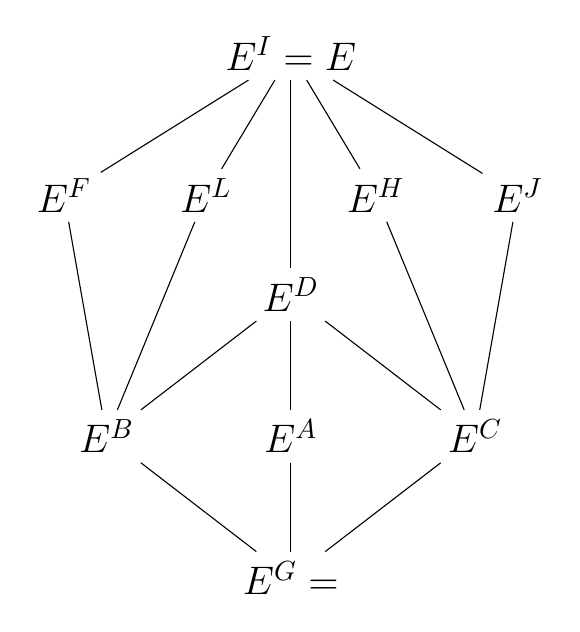
\begin{tikzpicture}[
	scale=1.8,
	every node/.style={font=\Large},
	yscale=-1
]
	\node (G) at (0,4) {$E^G = \Q$};
	\node (B) at (-1.3,3) {$E^B$} edge (G);
	\node (A) at (0,3) {$E^A$} edge (G);
	\node (C) at (1.3,3) {$E^C$} edge (G);
	\node (D) at (0,2) {$E^D$} edge (B) edge (A) edge (C);
	\node (F) at (-1.6,1.3) {$E^F$} edge (B);
	\node (L) at (-0.6,1.3) {$E^L$} edge (B);
	\node (H) at (0.6,1.3) {$E^H$} edge (C);
	\node (J) at (1.6,1.3) {$E^J$} edge (C);
	\node (I) at (0,0.3) {$E^I = E$} edge (F) edge (L) edge (D) edge (H) edge (J);
\end{tikzpicture}
}
			\caption{Fixkörper}
		\end{subfigure}
		\caption{Hierarchien der Untergruppen von $G(E / \Q)$, bzw. der Fixkörper von $E$}
		 \label{fig:19.5-5}
	\end{figure}

	Offenbar sind $I$ und $G$ Normalteiler von $G$.
	Die Untergruppen $B, A, C$ haben Index 2 in $G$ und sind daher Normalteiler von $G$.
	Das Zentrum von $G$, $Z(G) = D$ hat Index 4, ist aber ebenfalls normal in $G$, $G / D \isomorphic C_2 \times C_2$.
	Also sind die Fixkörper $E^A, E^B, E^C$ normal über $\Q$ mit Galoisgruppe $G / E^A, G / E^B, G / E^C \isomorphic C_2$ und $E^D$ ist normal über $\Q$ mit Galoisgruppe $G / D \isomorphic C_2 \times C_2$.

	Es gilt: $\sigma^{-1} L \sigma = F$ und $\sigma^{-1} J \sigma = H$, also sind $L, F, J, H$ keine Normalteiler und daher sind $E^L, E^F, E^J, E^H \subset E$ nicht normal über $\Q$.
	Trotzdem ist $E^L$ normal über $E^B$ und $E^B$ normal über $\Q$ wegen $2 = [E^L : E^B] = [E^B : \Q]$.
	Dies bestätigt, dass „normal über“ nicht transitiv ist, siehe auch \ref{19.3-4}.
\end{ex}


\section{Inseparable Körpererweiterungen}

Wir wollen uns zu guter letzt in diesem Kapitel nochmals inseparable Körpererweiterungen vorknöpfen und ihre Struktur genauer bestimmen.
Jetzt sei also $K$ ein unendlicher (wegen \ref{19.2-5}) Körper der Charakteristik $p > 0$ (wegen \ref{19.1-6}) und sei $K \subset E \subset \_K$ algebraische Körpererweiterung von $K$.

\begin{df} \label{19.6-1}
	Sei $\Char K = p > 0$.
	Dann heißt $\alpha \in \_K$ \emphdef{rein inseparabel} über $K$, falls $a^{p^n} \in K$ ist für ein $n \in \N$.
	\begin{note}
		So ist $\alpha \in \_K$ rein inseparabel genau dann, wenn $\beta \in K, n \in \N$ existieren mit $\alpha^{p^n} = \beta$, d.h. $\alpha$ Nullstelle von $x^{p^n} - \beta \in K[x]$.
		Also ist dann in $\_K[x]$
		\[
			x^{p^n} - \beta
			= x^{p^n} - \alpha^{p^n}
			= (x - \alpha)^{p^n},
		\]
		d.h. $\alpha$ ist Nullstelle von $x^{p^n} - \beta$ mit Vielfachheit $p^n$.
		Insbesondere besitzt dann der Teiler $\mu_{\alpha, K} \in K[x]$ ebenfalls nur die Nullstelle $\alpha$ mit Vielfachheit einer $p$-Potenz.
	\end{note}
\end{df}

\begin{df} \label{19.6-2}
	Sei $K \subset E \subset \_K$.
	Dann heißt \emphdef[rein inseparabel]{$E$ rein inseparabel über $K$}, falls $\alpha$ rein inseparabel über $K$ ist für alle $\alpha \in E$.
	\begin{note}
		$E$ besteht dann ausschließlich aus $p^n$-ten Wurzeln von Elementen aus $K$.
	\end{note}
\end{df}

\begin{st} \label{19.6-3}
	Sei $\Char K = p > 0$, $K \subset E \subset \_K$.
	Dann sind äquivalent:
	\begin{enumerate}[i)]
		\item
			$[E : K]_S = 1$,
		\item
			$E$ ist rein inseparabel über $K$,
		\item
			$\forall \alpha \in E \exists \beta \in K, n \in \N : \mu_{\alpha, K} = x^{p^n} - \beta \in K[x]$,
		\item
			es existiert $S = \{\alpha_i : i \in I$ mit $E = K(S)$ und $\alpha_i$ rein inseparabel über $K$ für alle $i \in I$,
		\item
			für alle $\alpha \in E, \alpha \not\in K$ ist $\alpha$ inseparabel über $K$.
	\end{enumerate}
\end{st}

\begin{st} \label{19.6-4}
	Sei $\Char K = p > 0$, $K \subset E \subset \_K$.
	Sei $E_S = \{ \alpha \in E : \text{\(\alpha\) separabel über \(K\)} \}$.
	Dann ist $E_S$ eine algebraische separable Körpererweiterung von $K$, der \emphdef{separable Abschluss} von $K$ in $E$ und $E$ ist rein inseparabel über $E_S$.
	Darüber hinaus gilt: $[E_S : K] = [E : K]_S$.
\end{st}

\begin{st} \label{19.6-5}
	Sei $K \subset E \subset \_K$ und sei $E$ normal über $K$.
	Dann ist auch der separable Abschluss von $K$ in $E$ normal über $K$ und daher galoissch über $K$ und es gilt $G(E / K) = G(E_S / K)$.
\end{st}

\begin{nt} \label{19.6-6}
	\ref{19.6-4} besagt also, dass man sich jede algebraische Körpererweiterung $E$ eines Körpers $K$ mit $\Char K = p > 0$ in zwei Schritten zerlegen kann:
	\begin{enumerate}[1.]
		\item
			bilden einer separablen Körpererweiterung $E_S$ von $K$,
		\item
			anschließendes adjungieren aller $p^k$-ten Wurzeln von Elementen aus $E_S$:
			\begin{align*}
				E &= E_S(T),&
				T &= \Set{ \alpha_i \in E & \exists r_i \in \N : \alpha_i^{p^{r_i}} \in E_S }.
			\end{align*}
	\end{enumerate}
	Betrachte beispielswiese $K = \F_p(t) = Q(\F_p[t]), E = K(\sqrt[p]{t})$.
\end{nt}





